\documentclass[9pt,english,utf8]{article}

\newcommand{\etal}{\emph{et al.}\@\xspace}

\usepackage{graphicx}
\usepackage{array}
\usepackage{enumerate}
\usepackage{booktabs}
\usepackage{subfigure}
\usepackage{amsmath}
\usepackage{units}
\usepackage{xspace}
\usepackage{caption}
\usepackage{xcolor}
\usepackage{cases}

\graphicspath{{figures/}}

\usepackage{tikz}
\usetikzlibrary{matrix,shapes,arrows,positioning,backgrounds,decorations.pathreplacing,shapes.misc,decorations.text}


\definecolor{a}{HTML}{FFB338}
\definecolor{b}{HTML}{FC6039}
\definecolor{c}{HTML}{FF194D}
\definecolor{d}{HTML}{F73CB5}
\definecolor{e}{HTML}{E63DF4}
\definecolor{f}{HTML}{A54CFF}
\definecolor{g}{HTML}{887FFF}
\definecolor{h}{HTML}{3379FF}
\definecolor{i}{HTML}{42C3E9}
\definecolor{j}{HTML}{43E7C7}
\definecolor{k}{HTML}{44E481}
\definecolor{l}{HTML}{4CE246}
\definecolor{m}{HTML}{43E795}
\definecolor{n}{HTML}{98E246}


\newcommand{\telstart}[2]{
    \pgfmathsetmacro{\x}{#1}
    \pgfmathsetmacro{\y}{#2}
    \fill[color=gray] (\x+0.18, \y+0.16) arc (90:270:0.16 and 0.16) -- (\x+0.18,
    \y+0.16);
}
\newcommand{\telend}[2]{
    \pgfmathsetmacro{\x}{#1}
    \pgfmathsetmacro{\y}{#2}
    \fill[color=gray] (\x, \y+0.16) arc (270:90:-0.16 and -0.16) -- (\x,
    \y+0.16);
}

\newcommand{\gene}[3]{
    \pgfmathsetmacro{\x}{#1}
    \pgfmathsetmacro{\y}{#2}
    \foreach \char [count=\ci] in #3 {
        \fill[draw=none,color=\char] (\x, \y +\ci*0.32 - 0.16) rectangle
        (\x+0.78, \y +\ci*0.32 - 0.48);
        \node[color=black] at (\x+0.39, \y + \ci*0.32 - 0.32) {\textbf{\small\char}};
    }
}
 


\title{Horizontal Gene Transfer Phylogenetics: A First Model-Based Approach\\
Simulation Experiments}
\begin{document}
\maketitle
%\tableofcontents

\section{Background}

In Equation~16 of the main manuscript, we proposed an empirically derived
estimator for the \emph{synteny index} (SI) and showed in simulation, that it
performs well under the studied model of \emph{horizontal gene transfer} (HGT).
Here, we use the inverse of the measure  with the aim to derive additive
distances:

\begin{equation}
     \hat t = d_{SI}^k(x) = \frac{-n}{\lambda (3-\frac{5k}{n-1})} \log(x)
\end{equation}

The goal of this experiment is to evaluate the SI distance in an applied
setting that is close to practice. Therefore, we simulate genome evolution of
multiple taxa that evolve under our HGT model. 

\paragraph{Genome evolution.} We used ALF\cite{Dalquen:2012dx} as genome
evolution simulator of phylogenies with more than two taxa. ALF supports
various genome rearrangement operations, one of which being
\emph{translocations}. Translocations, more commonly known as
\emph{transpositions}, permute the gene order by moving blocks of genes from
one genomic location to another. ALF provides parameters to limit the number of
genes that are transposed in one event. In accordance with our model, we set
this number to 1. By doing so, ALF's genome rearrangement model under
transpositions is equivalent to the HGT model underlying our study.
Counterbalancing the computation time with a realistic scenario, the number of
genes per genome in the simulations is set to 1000. In all simulations, we
chose the same evolutionary tree comprising 10 extant taxa. The tree has a
balanced layout, i.e., it is highly symmetric and all edges have the same
length (see Figure \ref{fig:tree}). To quantify the quality of reconstruction
under various evolutionary scenarios, we scaled the tree from small diameters
(0.5 PAM) to large (50 PAM) using a constant transposition rate of $0.01$. 

\paragraph{Experimental setup.}
First, we performed a simple experiment in reconstructing pairwise distances,
i.e.  estimating the true evolutionary time from SI measures. To this end, we
sampled 10 genome sequences comprising 1000 genes per time point and calculated
$\hat t = d_{SI}^k$ for different values of $k$.  

However, the main goal of this experiment is to assess the power of the SI
distance beyond the reconstruction of pairwise distances. That is, inferring
phylogenies comprising several taxa. The inverse SI being a \emph{distance}
measure we naturally followed standard procedure of distance-based
reconstruction. As tree reconstruction method, we chose \emph{Neighbor
Joining} (NJ), a classic and robust method for reconstructing unrooted trees.
The quality of the reconstruction is subsequently quantified by comparing the
topology of the reconstructed and the original tree using the classic
\emph{Robinson-Foulds} (RF) distance. Each measured point in time subsumes 500
sampled genomic datasets. 

\begin{figure}[tb]
    \centering 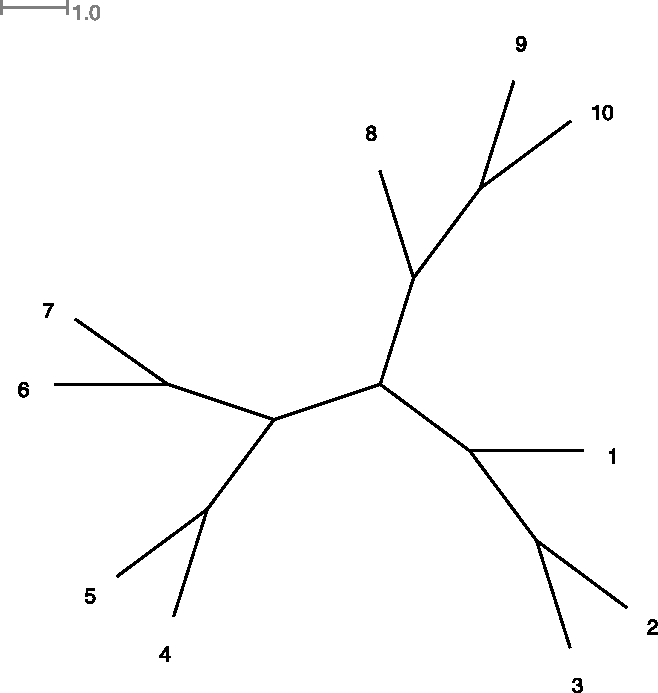
\includegraphics[width=0.3\columnwidth]{true_tree_s10_pam10}

    \caption{Phylogenetic tree of 10 taxa used in the simulation experiments.}
    \label{fig:tree}
\end{figure}

\paragraph{Results} The outcome of the experiment in pairwise distance
reconstruction is visualized in Figure~\ref{fig:results}~(a). Despite the
inverted SI being not truthful to the true time, it remains additive for a
large range of evolutionary time. This indicates that the measure is
well-suited for distance-based reconstruction of phylogenetic trees. 

Figure~\ref{fig:results}~(b) shows the outcome of the experiment of inferring
the 10 taxa comprising tree of Figure~\ref{fig:tree} from low to high numbers
of mutations (measured in PAM). The plot depicts well the two cases of poor
reconstruction under the studied HGT model: for low values of PAM, not enough
HGTs are taking place, whereas for large values of PAM, the gene order
sequences are saturated from the excess of HGT events. 

Next to the SI distance, we included the
double-cut-and-join (DCJ) distance for comparison. The DCJ distance is
parsimonious (i.e., non-additive) and the most prevalent measure used for
quantifying genome rearrangement. In our experiment, the inverted SI
outperforms the DCJ distance even for poor choices of $k$ (cf. $k=100$). 

\begin{figure}[tb]
    
    \subfigure[]{
    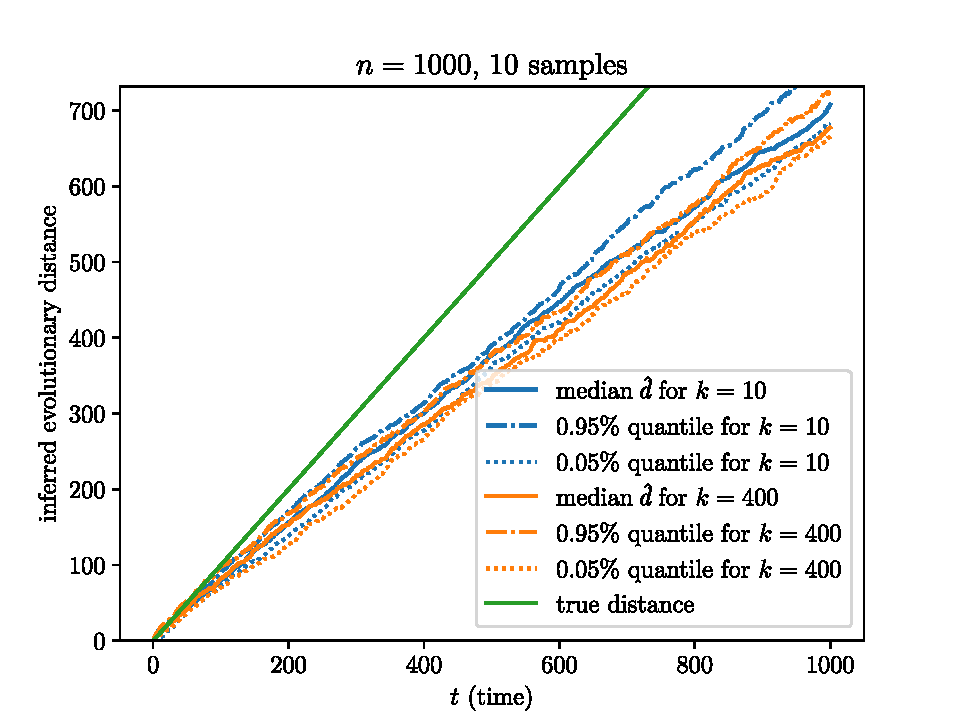
\includegraphics[width=0.5\columnwidth]{distance_plot_n1000_s10_inv}
    }
    \subfigure[]{
    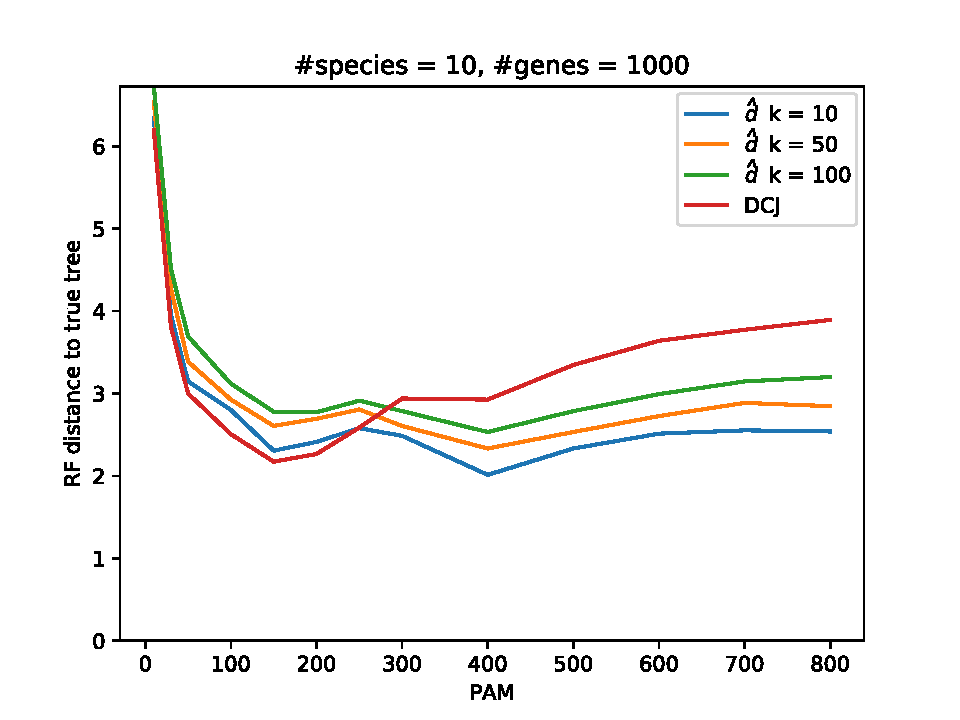
\includegraphics[width=0.5\columnwidth]{boxplot_s10_n1000}
    }

    \caption{\textbf{(a)} Median, $5\%$-, and $95\%$-quantiles of inferred
    pairwise distances $\hat t = d_{SI}$ for $k=10, 400$. \textbf{(b)} Mean RF
distances between the reconstructed and true trees of the simulation. }
\label{fig:results}
\end{figure}


\bibliographystyle{plain} 
\bibliography{references} 

\end{document}
